% !TEX root = ../thesis.tex

\chapter{Mikrosvety vo výučbe základov pro-gramovania}\label{ch:microworlds}

V roku 1967 vytvorila skupina výskumníkov okolo \emph{Seymour Paperta} z \emph{MIT} programovací jazyk určený pre výučbu programovania na školách s názvom \emph{LOGO}. Jazyk \emph{LOGO} sa tak stal prvým príkladom tzv. \textbf{mikrosveta} - jednoduchého, samostatného programovacieho prostredia určeného pre výučbu.

V rozličnej literatúre sa je možné stretnúť s rozličnými synonymami slova \emph{mikrosvet}. Napríklad \emph{Rudolf Pecinovský} v článku \cite{Pecinovsky2001} hovorí o \emph{virtuálnych svetoch}. Kolektív autorov v článku \cite{Brusilovsky} zasa okrem \emph{mikrosvetov} hovoria aj o \emph{mini jazykoch}. Všetci však stále pomenúvajú tie isté riešenia, ale zakaždým iným termínom. Pre potreby tejto práce budem používať termín \emph{mikrosvet}, ktorý zaviedol práve \emph{Seymour Papert}.

V tejto kapitole budú opísané vlastnosti \emph{mikrosvetov} a niektoré implementácie známe v našom regióne budú predstavené. Mikrosvet \emph{Robota Karla} bude predstavený v samostatnej kapitole \ref{ch:karel.the.robot}.


\section{Mikrosvet a jeho vlastnosti}

Prehľad rozličných definícií termínu \emph{mikrosvet} je možné nájsť v článku \cite{djelil:hal-02438255}. Samotný koncept \emph{mikrosveta} však zaviedol \emph{Seymour Papert} a svoje skúsenosti a teórie o vzdelávaní zhrnul vo svojej knihe \emph{Mindstorms} \cite{Papert1980}. Ten opísal \glslink{microworld}{mikrosvet} ako zjednodušené, samostatné prostredie navrhnuté tak, aby pomáhalo študentom skúmať a porozumieť špecifickým konceptom prostredníctvom priamej interakcie a experimentovania.

Používanie mikrosvetov v úvodných kurzoch programovania miesto štandarných programovacích jazykov má mnoho výhod. Niektoré z nich vymenoval \emph{Rudolf Pecinovský} vo svojom článku \cite{Pecinovsky2001}, iné je možné nájsť priamo  v knihe \cite{Papert1980} od \emph{Seymoura Paperta}. Niektoré z nich sú:

\begin{itemize}
    \item Mikrosvety sú \textbf{interaktívne} a \textbf{zábavné}. Riešenie úloh sa vykonáva na obrazovke pred študentmi, ktorí nepotrebujú explicitne pracovať so štandardným vstupom a výstupom.

    \item Mikrosvety poskytujú \textbf{okamžitú spätnú väzbu}. Okrem samotného výsledku vidí študent na obrazovke aj celú postupnosť krokov vedúcu k riešeniu problému. Vďaka tomu sa v programy jednoduchšie ladia a hľadajú sa v nich chyby.

    \item Mikrosvety ponúkajú \textbf{zjednodušené prostredie}. Komplexita veľkých jazykov je zjednodušená na niekoľko kľúčových slov a elementov, ktoré svet definujú. Tým pádom je možné vytvárať programy aj so začiatočníkmi už od prvých hodín. Rovnako je možné takmer okamžite predstaviť koncept procedúr/funkcií a následne predstaviť pravidlá dekompozície.
\end{itemize}

V súčasnosti existuje mnoho implementácií mikrosvetov, pomocou ktorých je možné viesť úvodné kurzy programovania. V nasledujúcich podkapitolách budú predstavené tri implementácie, ktoré sú známe v Čechách a na Slovensku od 80-tych rokov minulého storočia. Konkrétne bude predstavený jazyk \emph{LOGO} a čarodejník \emph{Baltík}. Tretiemu mikrosvetu - svetu Robota Karla - bude venovaná nasledujúca kapitola.



\section{Žofka a korytnačia grafika}

Ako už bolo uvedené, jazyk \emph{LOGO} je jedným z prvých programovacích jazykov určených na výučbu programovania. Program v jazyku \emph{LOGO} sa zapisuje pomocou textových príkazov, pričom tieto príkazy môžu byť priamo lokalizované do konkrétneho jazyka - či už programovacieho alebo jazyka konkrétnej krajiny. Vďaka tomu existuje mnoho implementácií tohto jazyka.

Mikrosvet jazyka \emph{LOGO} obsahuje kurzor, ktorým je korytnačka (u nás známa pod menom \emph{Žofka}). Korytnačka sa nachádza na plátne, je možné s ňou pohybovať a kresliť pomocou štetca. V počítačovej grafike je vďaka tomu známy termín \emph{korytnačia grafika}, ktorý reprezentuje vektorovú grafiku vytváranú práve korytnačkou.

Vo výpise \ref{lst:imagine.logo} sa nachádza kód napísaný v lokalizovanej verzii jazyka \emph{Imagine Logo} na vytvorenie vlastného príkazu \texttt{stvorce}. Výstup po zavolaní tohto príkazu je možné vidieť na obrázku \ref{fig:imagine.logo}.

\lstinputlisting[language={Logo},caption={Procedúra stvorce v jazyku Imagine Logo}]{listings/turtle.txt}\label{lst:imagine.logo}


\begin{figure}[htbp]
   \centering
   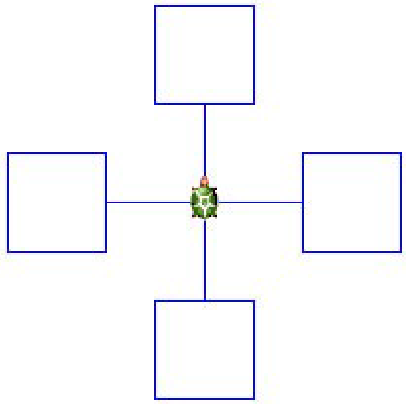
\includegraphics[width=.5\textwidth]{figures/imagine.logo.png}
   \caption[Výstup programu v jazyku Imagine Logo]{Výstup programu v jazyku Imagine Logo}
   \label{fig:imagine.logo}
\end{figure}


\section{Mladý čarodejník Baltík}

Grafický programovací jazyk \emph{Baltík}\footnote{\url{http://www.sgpsys.com/cz/Product_B3.asp}} vyvinula česká spoločnosť \emph{SGP Systems}\footnote{\url{http://www.sgpsys.com/cz/}} v roku 1996. Je určený na výuku programovania na základných a stredných školách.

Ako autori uvádzajú na domovskej stránke,  \emph{Baltík 3} sa stal vzorom pro mnoho známých nástrojov, akým je napríklad aj \emph{Scratch}\footnote{\url{https://scratch.mit.edu/}}. Ten vznikol na americkej univerzite \emph{MIT} zhruba 6 rokov po predstavení \emph{Baltíka} profesorovi Seymourovi Papertovi v roku 1998.

Na obrázku \ref{fig:baltik} sa nachádza príklad programu napísaný v jazyku \emph{Baltík}. Tento program sa skladá z troch riadkov, ktorých význam je nasledovný:

\begin{enumerate}
   \item Najprv Baltík vykoná 5-krát zložený príkaz, v ktorom najprv pred sebou zasadí strom a následne sa posunie o jedno políčko smerom doprava.

   \item V druhom riadku baltík postupne pred sebou postaví okno, spraví krok a postaví aj dvere. Následne urobí vľavo vbok a postaví pred sebou strechu. Následne urobí vpravo vbok, krok, vľavo vbok a postaví strechu s komínom.

   \item V poslednom riadku bude Baltík čakať na stlačenie klávesy alebo tlačidla myši.
\end{enumerate}

\begin{figure}[htbp]
   \centering
   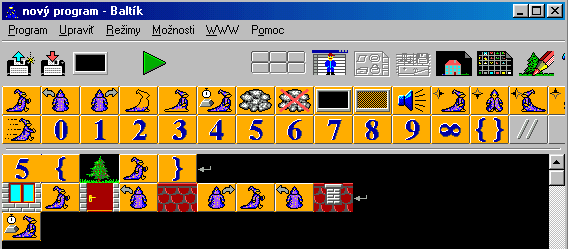
\includegraphics[width=.9\textwidth]{figures/baltik.png}
   \caption[Zoznam príkazov a program napísaný v programovacom jazyku Baltík v režime začiatočník]{Zoznam príkazov a program napísaný v programovacom jazyku Baltík v režime začiatočník \footnotemark }
   \label{fig:baltik}
\end{figure}

\footnotetext{Zdroj: \url{https://www.sgpsys.com/infovek/zakl_inf3.htm}}

